% Survey taxonomy: overlapping analytic dimensions, with benchmark examples.
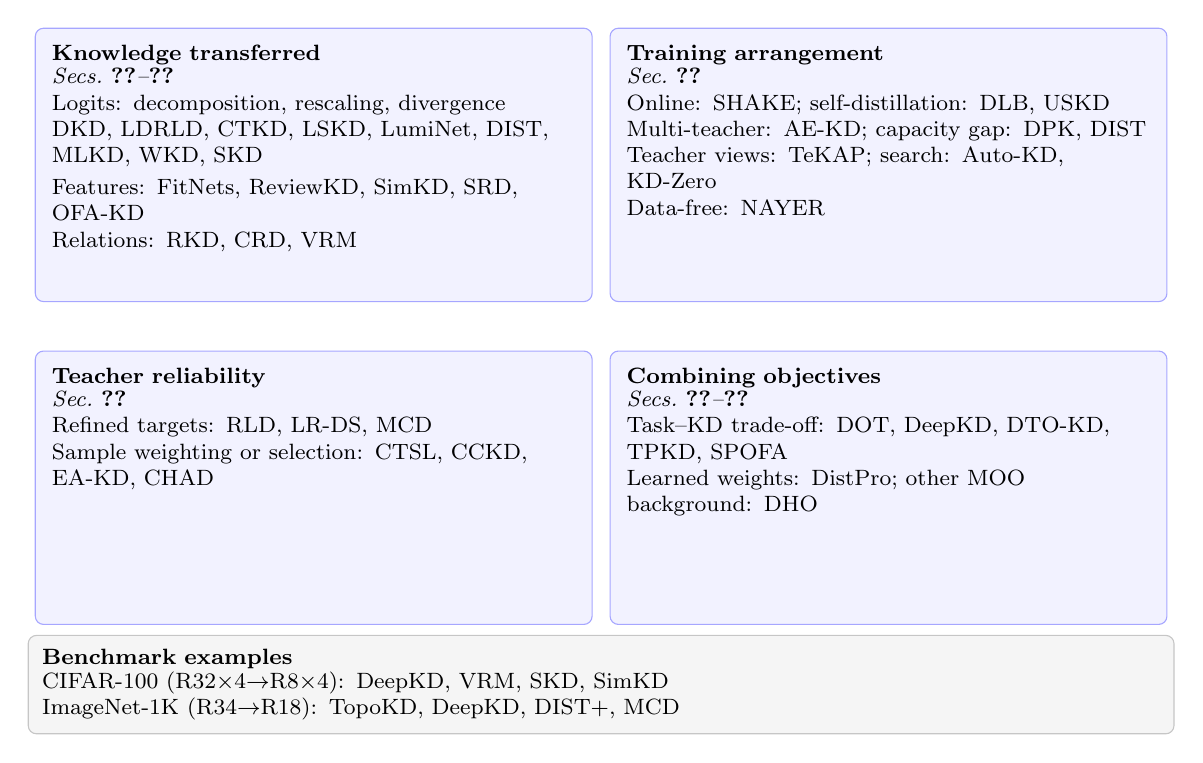
\begin{tikzpicture}[x=1cm,y=1cm,font=\footnotesize,
  card/.style={draw,rounded corners=3pt,fill=blue!5,draw=blue!35,
    text width=6.65cm,minimum height=3.45cm,inner sep=6pt,align=left},
  bench/.style={draw,rounded corners=3pt,fill=gray!8,draw=gray!45,
    text width=14.2cm,minimum height=1.05cm,inner sep=5pt,align=left}]
  \node[card] (knowledge) at (-3.65,2.05) {\parbox[t][3.05cm][t]{6.65cm}{\raggedright \textbf{Knowledge transferred}\\[-1pt]
    \textit{Secs.~\ref{sec:logit}--\ref{sec:feature}}\\
    Logits: decomposition, rescaling, divergence\\
    DKD, LDRLD, CTKD, LSKD, LumiNet, DIST, MLKD, WKD, SKD\\[2pt]
    Features: FitNets, ReviewKD, SimKD, SRD, \mbox{OFA-KD}\\
    Relations: RKD, CRD, VRM}};
  \node[card] (arrangement) at (3.65,2.05) {\parbox[t][3.05cm][t]{6.65cm}{\raggedright \textbf{Training arrangement}\\[-1pt]
    \textit{Sec.~\ref{sec:schemes}}\\
    Online: SHAKE; self-distillation: DLB, USKD\\
    Multi-teacher: AE-KD; capacity gap: DPK, DIST\\
    Teacher views: TeKAP; search: Auto-KD, \mbox{KD-Zero}\\
    Data-free: NAYER}};
  \node[card] (reliability) at (-3.65,-2.05) {\parbox[t][3.05cm][t]{6.65cm}{\raggedright \textbf{Teacher reliability}\\[-1pt]
    \textit{Sec.~\ref{sec:reliability}}\\
    Refined targets: RLD, LR-DS, MCD\\
    Sample weighting or selection: CTSL, CCKD, EA-KD, CHAD}};
  \node[card] (objectives) at (3.65,-2.05) {\parbox[t][3.05cm][t]{6.65cm}{\raggedright \textbf{Combining objectives}\\[-1pt]
    \textit{Secs.~\ref{sec:moo}--\ref{sec:kd_moo}}\\
    Task--KD trade-off: DOT, DeepKD, DTO-KD, TPKD, SPOFA\\
    Learned weights: DistPro; other MOO background: DHO}};
  \node[bench] (benchmarks) at (0,-4.55) {\textbf{Benchmark examples}\\[-1pt]
    CIFAR-100 (R32$\times$4$\to$R8$\times$4): DeepKD, VRM, SKD, SimKD\\
    ImageNet-1K (R34$\to$R18): TopoKD, DeepKD, DIST+, MCD};
\end{tikzpicture}
